%% packages
\documentclass{article}
\usepackage[a4paper, left=2.0cm, right=2.0cm, top=3.5cm]{geometry}
\usepackage[ngerman]{babel}
\usepackage{graphicx}
\usepackage{multicol}
\usepackage{amssymb}
\usepackage{titlesec}
\usepackage{wrapfig}
\usepackage{blindtext}
\usepackage{lipsum}
\usepackage{caption}
\usepackage{listings}
\usepackage{fancyhdr}
\usepackage{nopageno}
\usepackage{authblk}
\usepackage{amsmath} % tons of math stuff
\usepackage{mathtools} % e.g. alignment within matrix
%\usepackage{bm} % provides shorthand for bold in math mode
\usepackage{dsfont} % \mathds makes double stroke digits
\usepackage{esdiff} % provides \diff
%\usepackage[ISO]{diffcoeff}
\usepackage{xcolor}
\usepackage{csquotes} % e.g. provides \enquote
\usepackage[separate-uncertainty=true]{siunitx} % units
\usepackage{xcolor} % colored text
\usepackage[l3]{csvsimple}
\usepackage{subcaption}
\usepackage{physics}
\usepackage{hyperref}
\usepackage{nameref}
\hypersetup{colorlinks=true, linkcolor=black, pdfhighlight={/N}}
\usepackage{tcolorbox}
\usepackage{amsthm}
\usepackage{gensymb} % add \degree in math mode?
\usepackage{newunicodechar} % define custom unicode characters
\usepackage{booktabs}
\usepackage{subcaption}

% \sisetup{
%   scientific-notation = auto,  % Automatically use scientific notation for large/small numbers
%   output-exponent-marker = \text{e}  % (optional) for formatting the exponent symbol
% }



%\fancyhf[]{}

%% custom stuff
% own units
\DeclareSIUnit \VSS {\ensuremath{V_\mathrm{SS}}}
\DeclareSIUnit \VS {\ensuremath{V_\mathrm{S}}}
\DeclareSIUnit \Veff {\ensuremath{V_\mathrm{eff}}}
\DeclareSIUnit \Vpp {\ensuremath{V_\mathrm{pp}}}
\DeclareSIUnit \Vp {\ensuremath{V_\mathrm{p}}}
\DeclareSIUnit \VRMS {\ensuremath{V_\mathrm{RMS}}}
\DeclareSIUnit \ASS {\ensuremath{A_\mathrm{SS}}}
\DeclareSIUnit \AS {\ensuremath{A_\mathrm{S}}}
\DeclareSIUnit \Aeff {\ensuremath{A_\mathrm{eff}}}
\DeclareSIUnit \App {\ensuremath{A_\mathrm{pp}}}
\DeclareSIUnit \Ap {\ensuremath{A_\mathrm{p}}}
\DeclareSIUnit \ARMS {\ensuremath{A_\mathrm{RMS}}}

% change subsection numbering to capital letters
\newcommand{\subsectionAlph}{ \renewcommand{\thesubsection}{\arabic{section}.\Alph{subsection}} }
% change subsection numbering to lowercase letters
\newcommand{\subsectionalph}{ \renewcommand{\thesubsection}{\arabic{section}.\alph{subsection}} }
% change subsubsection numbering to lowercase letters
\newcommand{\subsubsectionalph}{ \renewcommand{\thesubsubsection}{\arabic{section}.\arabic{subsection}.\alph{subsubsection}} }
% own fig. that works with multicols
\newenvironment{Figure}
  {\par\medskip\noindent\minipage{\linewidth}}
  {\endminipage\par\medskip}
\newcommand*{\inputPath}{./plot} % prepend this command to the argument of all input commands
\newcommand*{\tablePath}{../data} % prepend this command to the argument of all input commands
\graphicspath{ {./figure/}{../plot/}{../assets} }
% own enviroment for definitions
\newenvironment{definition}[1]
{\begin{quote} \noindent \textbf{\textit{#1\ifx&#1& \else : \fi}} \itshape}
{\end{quote}}

\newunicodechar{°}{\degree}


% own commands
% \newcommand{\rarr}{$\to\,$} %A$\,\to\,$B
\newcommand{\defc}{black}
\newcommand{\colorT}[2][blue]{\color{#1}{#2}\color{\defc}}
\newcommand{\redq}{\color{red}(?)\color{\defc}}
\newcommand{\question}[1]{\colorT[purple]{\textbf{(#1)}}}
\newcommand{\todo}[1]{\colorT[red]{\textbf{(#1)}}}
\newcommand{\mr}{\mathrm}

%% preparation
\begin{titlepage}
    \title{Praktikum Atome, Moleküle, kondensierte Materie \\ Versuch 442: Laser}
    \author[1]{Michael Vogt\thanks{s65mvogt@uni-bonn.de}}
    \affil[1]{Uni Bonn}
    %\date{\today}
\end{titlepage}


%% document
\begin{document}

\pagenumbering{gobble}
\maketitle
\tableofcontents
\newpage
\pagenumbering{arabic}

\pagestyle{fancy}
\fancyhead[R]{\thepage}
\fancyhead[L]{\leftmark}

\section*{TODO}
\begin{itemize}
  \item \todo{\enquote{Aufgaben} durchgehen und ins Protokoll aufnehmen}
  
\end{itemize}

\section*{Einleitung}
Durch diesen Versuch soll die grundlegende Funktionsweise von Lasern anhand eines Helium-Neon-Lasers verstanden werden.
Zunächst werden Wellenlänge und Polarisation des Lichts gemessen und anschließend die Aufspaltung in verschiedene
Moden genauer untersucht. Zum stabilen Betrieb des Lasers wird eine optische Diode aufgebaut.

\section{Aufbau des Lasers}
Zunächst wird der Laser aufgebaut und justiert. Seine fundamentalen Bestandteile sind
\begin{enumerate}
  \item das \textbf{Lasermedium}, ein mit HeNe gefülltes Volumen. Durch Anlegen einer hohen Spannung kann das Helium
  auf den $2^1S_0$-Zustand angeregt und seine Energie durch inelastische Stöße an Neon-Atome abgeben,
  welche dadurch auf den 3s-Zustand, der ein ähnliches Energieniveau hat, angeregt werden (siehe Abb. \ref{fig:hene-level}).
  Dieser Zustand ist metastabil bezüglich spontaner Emission, wodurch es zu einer \textit{Besetzungsinversion} kommt: 
  Es befinden sich mehr Atome im höheren 3s-Zustand als im Grundzustand.
  \todo{Laserübergang beschreiben}
  % durch stimulierte Emission
  % kann jedoch der 3s$\rightarrow$2p-Übergang sehr häufig stattfinden.
  Dieser Prozess wird als \textbf{optisches Pumpen} bezeichnet.
  \item Ein \textbf{Resonator} aus zwei Spiegeln, der einen großen Teil des entstehenden Lichts vielfach durch das
  Lasermedium leitet. Dadurch können Photonen des 3s$\rightarrow$2p-Übergangs, der sonst nur selten durch
  spontane Emission stattfinden würde, denselben Übergang wieder
  stimulieren und weitere Photonen freisetzen. Es findet also ein verstärkender Prozess statt, der dem Laser
  seinen Namen gibt: \textit{Light Amplification Through Stimulated Emission of Radiation}.
\end{enumerate}

\begin{figure}[h]
  \centering
  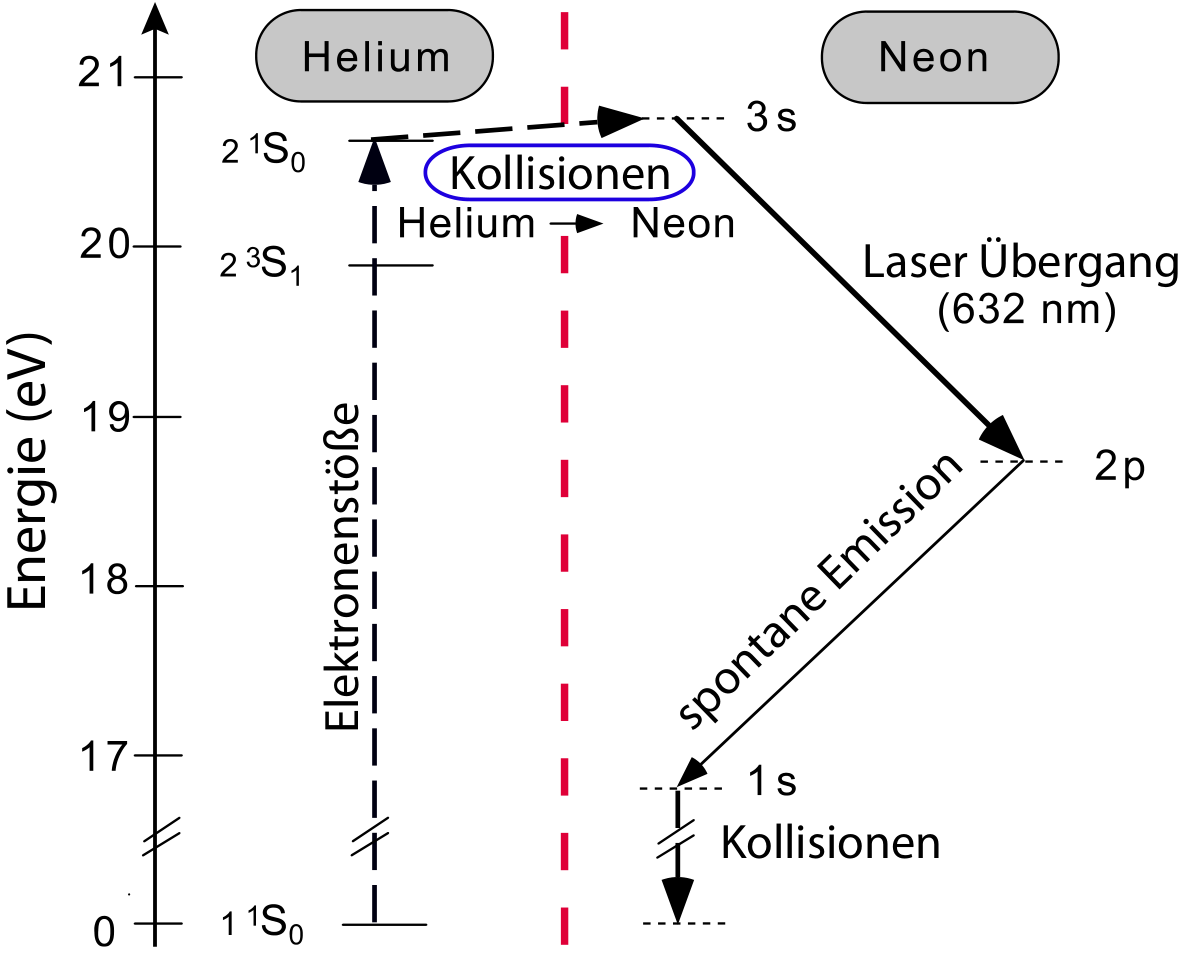
\includegraphics[width=0.5\textwidth]{hene-level}
  \caption{Für den Laserbetrieb relevant Energienievaus von Helium und Neon. \cite{Anleitung}}
  \label{fig:hene-level}
\end{figure}

\section{Wellenlänge und Polarisation}
Zunächst werden Wellenlänge und Polarisation des Laserlichts gemessen.
Es wurde ab hier ein anderer Aufbau als der zuvor beschriebene verwendet, da ich am zweiten Tag den Versuch als Teil
einer Dreiergruppe fortführte.
Die Aufbauten funktionieren grundlegend gleich und unterscheiden sich nur in den Details der Strahlführung.

\subsection{Wellenlänge}
Anhand der Ablenkung des Laserlichts an einem Transmissionsgitter, welches in den Strahlverlauf gestellt wird,
kann dessen Wellenlänge bestimmt werden.
Es gilt die Gittergleichung
\begin{equation}
  \lvert n \rvert\lambda = g(\cos \alpha - \cos \beta_n)
\end{equation}
wobei $\alpha$ der Winkel des Lasers und $\beta_n$ der Winkel der $n$-ten Beugungsordnung zur Gitternormalen ist
und $g = \frac{1}{600}\si\mm$ für die Gitterkonstante steht. 
Daraus folgt die Geradengleichung
\begin{equation}
  \lvert n \rvert = f(\cos\beta) = \frac{g}{\lambda} (\cos \alpha - \cos \beta)
\end{equation}
also gilt für die Steigung $m$
\[
  m = -\frac{g}{\lambda} \iff \lambda = -\frac{g}{m}
\]

\todo{Winkel aus Abstand berechnung}
Die gemessenen Ordnungen sind in Tab. \ref{tab:gitter-fit} gezeigt.

\begin{table}[h]
  \centering
  \begin{tabular}{c}
    \todo{werte}
  \end{tabular}
  \caption{
    Gemessene Ordnungen der Beugung des Laserlichts am Gitter. Die Position $x=0$ der 0-ten Ordnung folgt
    daraus, dass alle anderen $x$-Werte jeweils als Abstand zur 0-ten Ordnung gemessen wurden.
  }
\end{table}

Eine Geradenanpassung von $n$ in Abhängigkeit von $\cos \beta$ liefert die Gleichung
\[
  n = \todo{Werte}
\]
also $m = \todo{Wert}$ und $\lambda = \todo{Wert}$. \todo{Vergleich mit erwarteter Wellenlänge} 

\subsection{Polarisation}
Als nächstes soll die Polarisierung des Laserlichts gemessen werden. Im Lasermedium wird zunächst unpolarisiertes Licht
erzeugt. Dieses verlässt das Medium jedoch durch Brewsterfenster, welche nur eine bestimmte Polarisationsrichtung durchlassen

Brewsterfenster sind Fenster, die in ihrem Brewsterwinkel zur optischen Achse stehen. Dies ist der Winkel, bei dem
zur Einfallsebene parallel polarisiertes Licht vollständig transmittiert und nicht reflektiert wird.
Dazu senkrecht polarisiertes Licht wird sowohl transmittiert als auch reflektiert. Der reflektierte Anteil
verlässt die optische Achse und geht damit verloren.
Ein Brewsterfenster an sich lässt also eine Polarisationsrichtung stärker hindurch. Wird die andere Polarisationsrichtung
stark genug abgeschwächt (d.h. geht genug davon durch Reflexion verloren), reicht ihre Intensität
im Resonator nicht mehr aus, um den Laser zu betreiben.
So produziert der Laser im Idealfall nur Licht einer bestimmten Polarisationsrichtung.

Zur Messung der Polarisation wird das Licht durch einen Polarisator auf eine Photodiode geschickt
und die zur Lichtintensität proportionale Spannung mithilfe eines Oszilloskops gemessen.
Bei vollständig linear polarisiertem Licht und einem idealen Polarisator
ist der Zusammenhang zwischen Intensität $I$ und Winkel $\alpha$ des
Polarisators zur Vertikalen durch das \textit{Malus'sche Gesetz} gegeben:
\todo{ZITIEREN!!! BEI ALLEN FORMELN SCHAUEN}
\begin{equation}
  I(\alpha) = U_\mr{min} + (U_\mr{max}-U_\mr{min}) \cos^2(\alpha - \alpha_0) \label{eq:malus-real}
\end{equation}
Hier wurde Spannung $U$ anstatt Intensität $I$ verwendet, da die Spannung hier die
zur Intensität proportionale gemessene Größe ist.

Bei Sättigung der Diode würde der $\cos^2$-Verlauf oberhalb der Maximalspannung der Diode \enquote{abgeschnitten} werden
und damit nicht mehr \eqref{eq:malus-real} entsprechen. Es wurde daher sichergestellt, dass keine Sättigung auftritt.
Bei zu hoher Intensität kann die Diode mit einem BNC T-Stück mit einem \SI{50}{\ohm}-Abschlusswiderstand an einem Ausgang 
verbunden werden.
Der Polarisator auf verschiedene Winkel in regelmäßigen Abständen eingestellt und jeweils die Spannung notiert.
Diese Werte sind in Tab. \ref{tab:polarisation} gezeigt und in Abb. \ref{fig:polarisation} aufgetragen, zusammen
mit einer $\chi^2$-Anpassung nach \eqref{eq:malus-real}.
\begin{figure}[h]
  \begin{minipage}{0.49\textwidth}
    \centering
    \begin{tabular}{c|c}
  $\phi/\degree$ & $U/\si\mV$ \\
  \hline
  0 & 2.5 \\
  20 & 0.2 \\
  40 & 0.0 \\
  60 & 1.7 \\
  80 & 4.9 \\
  100 & 8.0 \\
  120 & 9.8 \\
  140 & 8.9 \\
  160 & 6.3 \\
  180 & 2.8 \\
  200 & 0.2 \\
  220 & 0.0 \\
  240 & 2.0 \\
  260 & 5.4 \\
  280 & 8.3 \\
  300 & 10.0 \\
  320 & 8.8 \\
  340 & 6.5 \\
\end{tabular}
    \caption{Spannung $U$ der Photodiode in Ab\-hängig\-keit der Richtung $\alpha$ des Polarisators zur Vertikalen.}
    \label{tab:polarisation}
  \end{minipage}
  \begin{minipage}{0.49\textwidth}
    \centering
    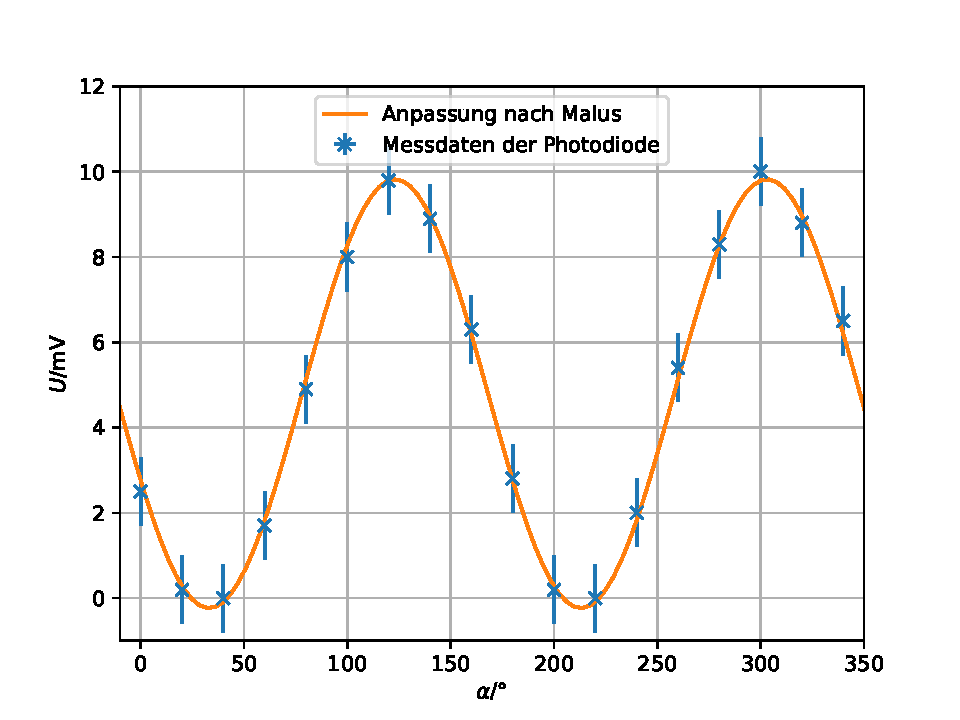
\includegraphics[width=\textwidth]{5.4polarisation}
    \caption{
      Spannung $U$ der Photodiode aufgetragen gegen den Winkel $\alpha$ des Polarisators.
      Daran wurde der Zusammenhang \eqref{eq:malus-real} angepasst.}
    \label{fig:polarisation}
  \end{minipage}
\end{figure}

Diese liefert die Parameter $\alpha_0 = \SI{123.09\pm0.36}{\degree}$,
$U_\mr{min} = \SI{-0.233\pm0.076}{\mV}$ und $U_\mr{max} = \SI{9.82\pm0.076}{\mV}$.

Der Winkel, in dem die Brewsterfenster stehen, wurde nicht exakt gemessen,
aber der hier bestimmte Wert für $\alpha_0$ scheint plausibel in Anbetracht der
bei der Durchführung beobachteten Drehstellung der Fenster.

Eine negative Spannung wie der hier bestimmte Wert für $U_\mr{min}$ entspricht einer negativen
Lichtintensität und ist damit unphysikalisch. Dass der Wert negativ ist kann ein Artefakt des Fits sein,
oder die Spannung wurde durch die Verbindung zwischen Diode und Oszilloskop verfälscht. Die gemessene
Spannung war relativ empfindlich gegen äußere Einflüsse wie z.B. Berührung des Kabels oder der Oszilloskops.
Das Signal war außerdem mit signifikanten Rauschen behaftet, Was zu einem Oszilloskop-Bild mit einer relativ
dicken Linie führte. Zum Ablesen wurde sich am unteren Rand dieser Linie orientiert,
was eine systematische Verschiebung zu kleineren Werten mit sich brachte. Diese beträgt schätzungsweise bis zu $\SI{0.4}{\mV}$

% % Der Polarisationsgrad PG ist definiert durch 
% % \begin{equation}
% %   \mr{PG} \coloneq \frac{I_\parallel - I_\perp}{I_\parallel + I_\perp}
% %   = \frac{U_\parallel - U_\perp}{U_\parallel + U_\perp}
% %   = \frac{U_\mr{max} - U_\mr{min}}{U_\mr{max} + U_\mr{min}} 
% % \end{equation}

Für den Polarisationsgrad PG gilt 
\begin{equation}
  \mr{PG} = \frac{U_\mr{max} - U_\mr{min}}{U_\mr{max} + U_\mr{min}} = \num{1.049\pm0.016}
\end{equation}
Dass der Polarisationsgrad größer als $1$ ist, wird durch das negative $U_\mr{min}$ versursacht.
Auch mit Berücksichtigung der systematischen Verschiebung würde sich jedoch kein Wert ergeben,
der weit unter $1$ liegt. Damit ist das Laserlicht, wie erwartet, vollständig polarisiert.
Abweichungen des gemessenen Polarisationsgrads von $PG=1$ könnten dadurch auftreten, dass der Polarisator nicht ideal ist.

% % Abweichungen von $PG=1$ könnten dadurch auftreten, dass im Lasermedium unabhängig von der Verstärkung durch den
% % Resonator auch die senkrechte Polarisationsrichtung erzeugt wird, wovon ein Teil durch die Brewsterfenster und

\section{Strahlprofil}
Als nächstes soll das Strahlprofil des Lasers, d.h. der Strahlradius $w$ in Abhängigkeit der Position $z$ 
entlang der optischen Achse, durchmessen werden.

In Resonatoren mit sphärischen Spiegeln entstehen sog. Gauß-Strahlen. Dies sind Lichtsstrahlen, deren transversales
(senkrecht zur optischen Achse) Intensitätsprofil die Form einer Gauß-Funktion hat.
Gauß-Strahlen sind in der Mitte zwischen den sphärischen Spiegeln am dünnsten. In unserem Fall werden nicht
zwei sphärische Spiegel, sondern ein sphärischer und ein planarer Spiegel verwendet.
Dieser Aufbau (\enquote{halbsymmetrischer Resonator} \cite{Anleitung}) ist äquivalent
zu einem Resonator doppelter Länger mit zwei sphärischen Spiegeln. 

Um die Breite eines Gauß-Strahls an einem bestimmten Punkt $z$ zu charakterisieren,
wird der Strahlradius $w$ definiert als der Radius (Abstand zur optischen Achse),
bei dem das elektrische Feld auf das $e^{-1}$-Fache seines Maximalwerts gefallen ist.
Der Strahlradius verhält sich in Abhängigkeit von $z$ nach dem Zusammenhang
\begin{equation}
  w(z) = w_0 \sqrt{1+\left( \frac{z}{z_R} \right)^2} \cite{Anleitung}
\end{equation}
Dabei ist $z$ der Abstand zur Strahltaille, dem Ort minimaler Strahldicke, und $w_0$ der Strahlradius bei der Strahltaille.
$z_R$ ist sie \textit{Raileigh-Länge} $z_R = \frac{\pi w_0^2}{\lambda}$

Für einen halbsymmetrischen Resonator ergibt sich der minimale Strahlradius durch
\begin{equation}
  w_0 = \sqrt{\frac{\lambda}{\pi} \sqrt{L(R-L)}} \cite{Anleitung}
\end{equation}
mit $\lambda$ der Wellenlänge, $L$ dem Abstand der Spiegel und $R$ dem Krümmungsradius des Hohlspiegels.

Die Messung der Breite des Strahls erfolgt, wie in der Versuchsanleitung beschrieben:
\blockquote{
  Für die Messung des Strahlradius w(z) verwenden Sie einen Messschieber. Dieser wird auf ca. 1.5 mm eingestellt und in den Strahlengang gebracht.
  Beachten Sie dabei, dass Sie nur den unteren, keilförmig zulaufenden Bereich der Messschieberbacken verwenden, um Messfehler zu vermeiden.
  Durch eine Bewegung des Messschiebers senkrecht zum Strahl
  blockt man somit den Laser entweder komplett oder verursacht Verluste durch teilweises Abschneiden des Strahls an den Messbacken.
  Ist der Abstand der Messbacken hinreichend groß, wird der Laser somit durch eine periodische Bewegung
  senkrecht zum Strahl in einem gepulsten Modus betrieben: Der Laser erlischt, wenn der Strahl verdeckt wird und blitzt auf,
  sobald der Strahl zwischen den Messbacken passieren kann. Ist der Abstand der Messbacken andererseits hinreichend klein,
  so sind die verursachten Verluste für den Laserbetrieb immer so groß, dass der Laser nicht arbeitet und der Laser bleibt
  stets dunkel. Die kleinste öffnung des Messschiebers, bei der noch Lasertätigkeit zu beobachten ist,
  ist demnach ein Maß für die Strahlgröße w(z). 
  
  [...] Eine andere Messmethode -- die von vielen Experimentatoren als simpler und robuster eingestuft wird -- besteht darin, 
  den Abstand der Messbacken zu fixieren um hierauf die axiale Position (entlang der Resonatorachse) des Messschiebers
  so lange zu verändern, bis das Aufblitzen des Lasers gerade nicht mehr zu beobachten ist.
  Die Messung wird mit verschiedenen sinnvollen Abständen der Messbacken wiederholt.
  \cite{Anleitung}
} 
\todo{Anleitung korrekt zitieren?}
In der Anleitung werden zwei verschiedene Messmethoden beschrieben, die jedoch auf dem gleichen Prinzip basieren,
dass die Breite des Strahls gemessen werden kann durch die Breite einer Öffnung, ab der nicht mehr genug Licht hindurchgelassen
wird, um den Laser zu \enquote{zünden}. In der Durchführung wurden beide Methoden eingesetzt, je nachdem,
was im konkreten Fall einfacher erschien.

Die Breite, die man durch diese Messmethode erhält, entspricht nicht dem Strahlradius, ist aber proportional zu ihm.
Zur Unterscheidung zum Strahlradius $w(z)$ werden die Messwerte im Folgenden mit $W(z)$ bezeichnet.

\todo{Werte und Tabellen und Plots und alles einfügen}


\section{Spektrum}
Schließlich soll das Spektrum des Lasers analysiert werden. Dieses wird bestimmt durch
\begin{enumerate}
  \item Die schwingenden Moden. Neben den longitudinalen Moden, welche durch die Länge des Resonators bestimmt werden,
    gibt es verschiedene transversale Moden. Diese unterscheiden sich im transversalen Profil das Laserlichts und
    können unterschiedliche Frequenzen haben.
  \item Die Linienbreite einzelner Moden. Durch Dopplerverbreiterung hat das Licht einer Mode
    einen ausgedehnten Frequenzbereich, welcher breit genug sein kann, um mehrere freie Spektralbreiten des
    Laserresonators zu überdecken. Dadurch werden aus dem Laser mehrere Linien, die den von der Mode
    überdeckten Transmissionsmaxima des Resonators entsprechen, ausgekoppelt.
    \todo{Die Aufspaltung ist wahrscheinlich so klein dass man sie nicht sieht}
\end{enumerate}
\todo{stimmt das? FSR erklären}

\subsection{optische Diode}
Da die Messung des Spektrums empfindlich ist, sollte der Laser hier möglichst stabil laufen.
Eine Quelle von Instabilität ist die Reflexion von ausgekoppeltem Licht zurück in den Laser. 
Dieses Licht interferiert mit dem Licht im Lasermedium und kann beeinflussen, welche Moden schwingen.

Um dies zu verhindern, wird eine optische Diode eingebaut, die Licht nur in einer Richtung hindurchlässt.
Sie besteht aus einem Polarisator hinter dem Planspiegel des Laserresonators und einer Verzögerungsplatte.
Zunächst wird der Polarisator eingebaut und so gedreht, dass er der Polarisationsrichtung des Laserlichts entspricht.
Dazu wird er zunächst so gedreht, dass die Transmission (nach Beobachtung mit dem Auge) minimal wird,
und dann um \ang{90} verstellt.

Dann werden die Verzögerungsplatte und dahinter ein Spiegel eingesetzt.
Die Platte kann entlang zwei Achsen verstellt werden und wird justiert, bis die rückreflektierte
Lichtintensität zwischen Polarisator und Planspiegel des Resonators minimal ist. Dies bedeutet,
dass die Verzögerungsplatte als $\lambda/4$-Platte agiert, welche im Winkel \ang{45} zur Polarisationsrichtung
der Laserlichts steht. dadurch wird das Laserlicht hinter der Platte zirkular polarisiert. Nach Reflexion
am Spiegel und erneutem Durchlaufen der Verzögerungsplatte ist es wieder linear polarisiert,
jedoch senkrecht zur vorigen Richtung. Dadurch kann das Licht den Polarisator nicht mehr passieren.

\subsection{Spektrumanalysator}
Die erste hier verwendete Messmethode verwendet einen sogenannten Spektrumanalysator.
Dies ist ein konfokaler Resonator mit einem Spiegelabstand $l=\SI{5}{\cm}$, der durch einen Piezo geringfügig verändert werden kann.
Die Längenänderung ist dabei (näherungsweise) proportional zur angelegten Spannung.
Die Mode $q$, $n$, $m$ hat die Frequenz
\begin{equation}
  \nu_{qnm} = \left(q + \frac{n + m}{2}\right)\frac{c}{2l}
\end{equation}
% Der Resonator transmittiert das Licht des Lasers, wenn dessen Frequenz einer seiner Moden entspricht.%, also $\nu_{qnm} = \nu$.
Der Modenabstand zwischen transversalen Moden ist also $\mr{MD} = \frac{c}{4l} = \SI{1499}{\MHz}$.
Der Resonator transmittiert das Licht des Lasers, wenn dessen Frequenz einer seiner Moden entspricht.
Durch Variation der Länge $l$ und Auftragen der entsprechenden Transmission lässt sich also das Spektrum des Lasers abbilden.

Hierzu wird am Piezo eine Wechselspannung (\SI{50}{\Hz}) angelegt.
Eine dazu proportionale Spannung wird an den x-Eingang und die Spannung einer Photodiode hinter
dem Analysator an den y-Eingang eines Oszilloskops im xy-Modus gegeben.
Die resultierenden Bilder für zwei verschiedene Laserresonatorlängen sind in Abb. \ref{fig:analysator} gezeigt.
\begin{figure}[h]
  \centering
  \begin{subfigure}{0.49\textwidth}
    \centering
    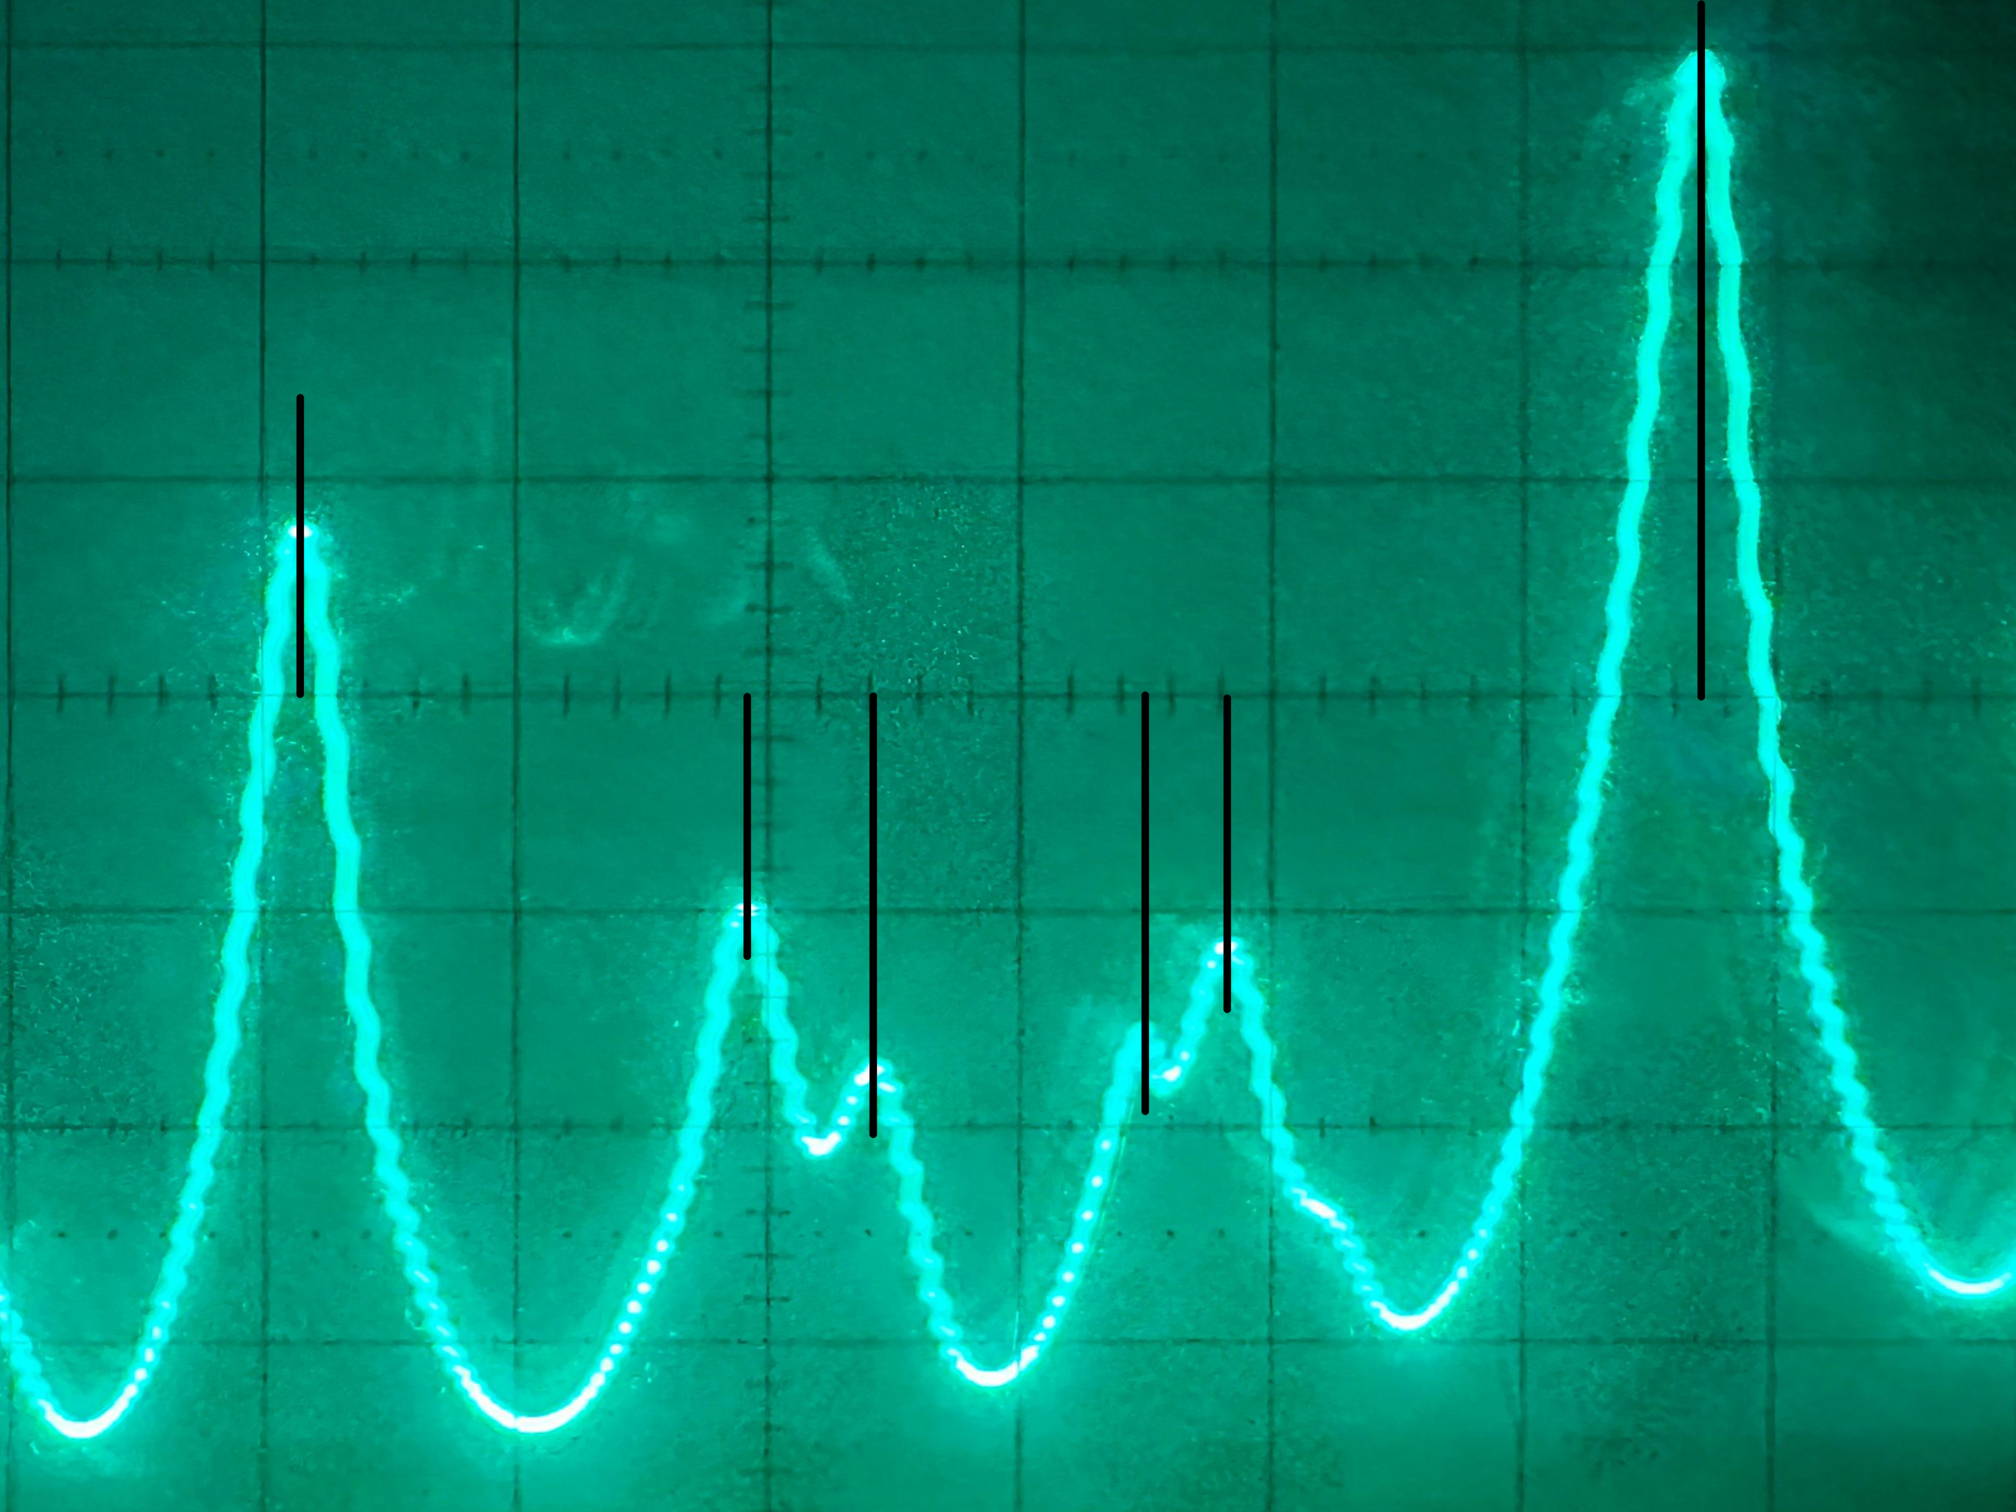
\includegraphics[width=\textwidth]{analysator-kurz}
    \subcaption{mit Laserresonator der Länge L=\SI{48.6}{\cm}.}
    \label{fig:analysator-kurz}
  \end{subfigure}
  \hfill
  \begin{subfigure}{0.49\textwidth}
    \centering
    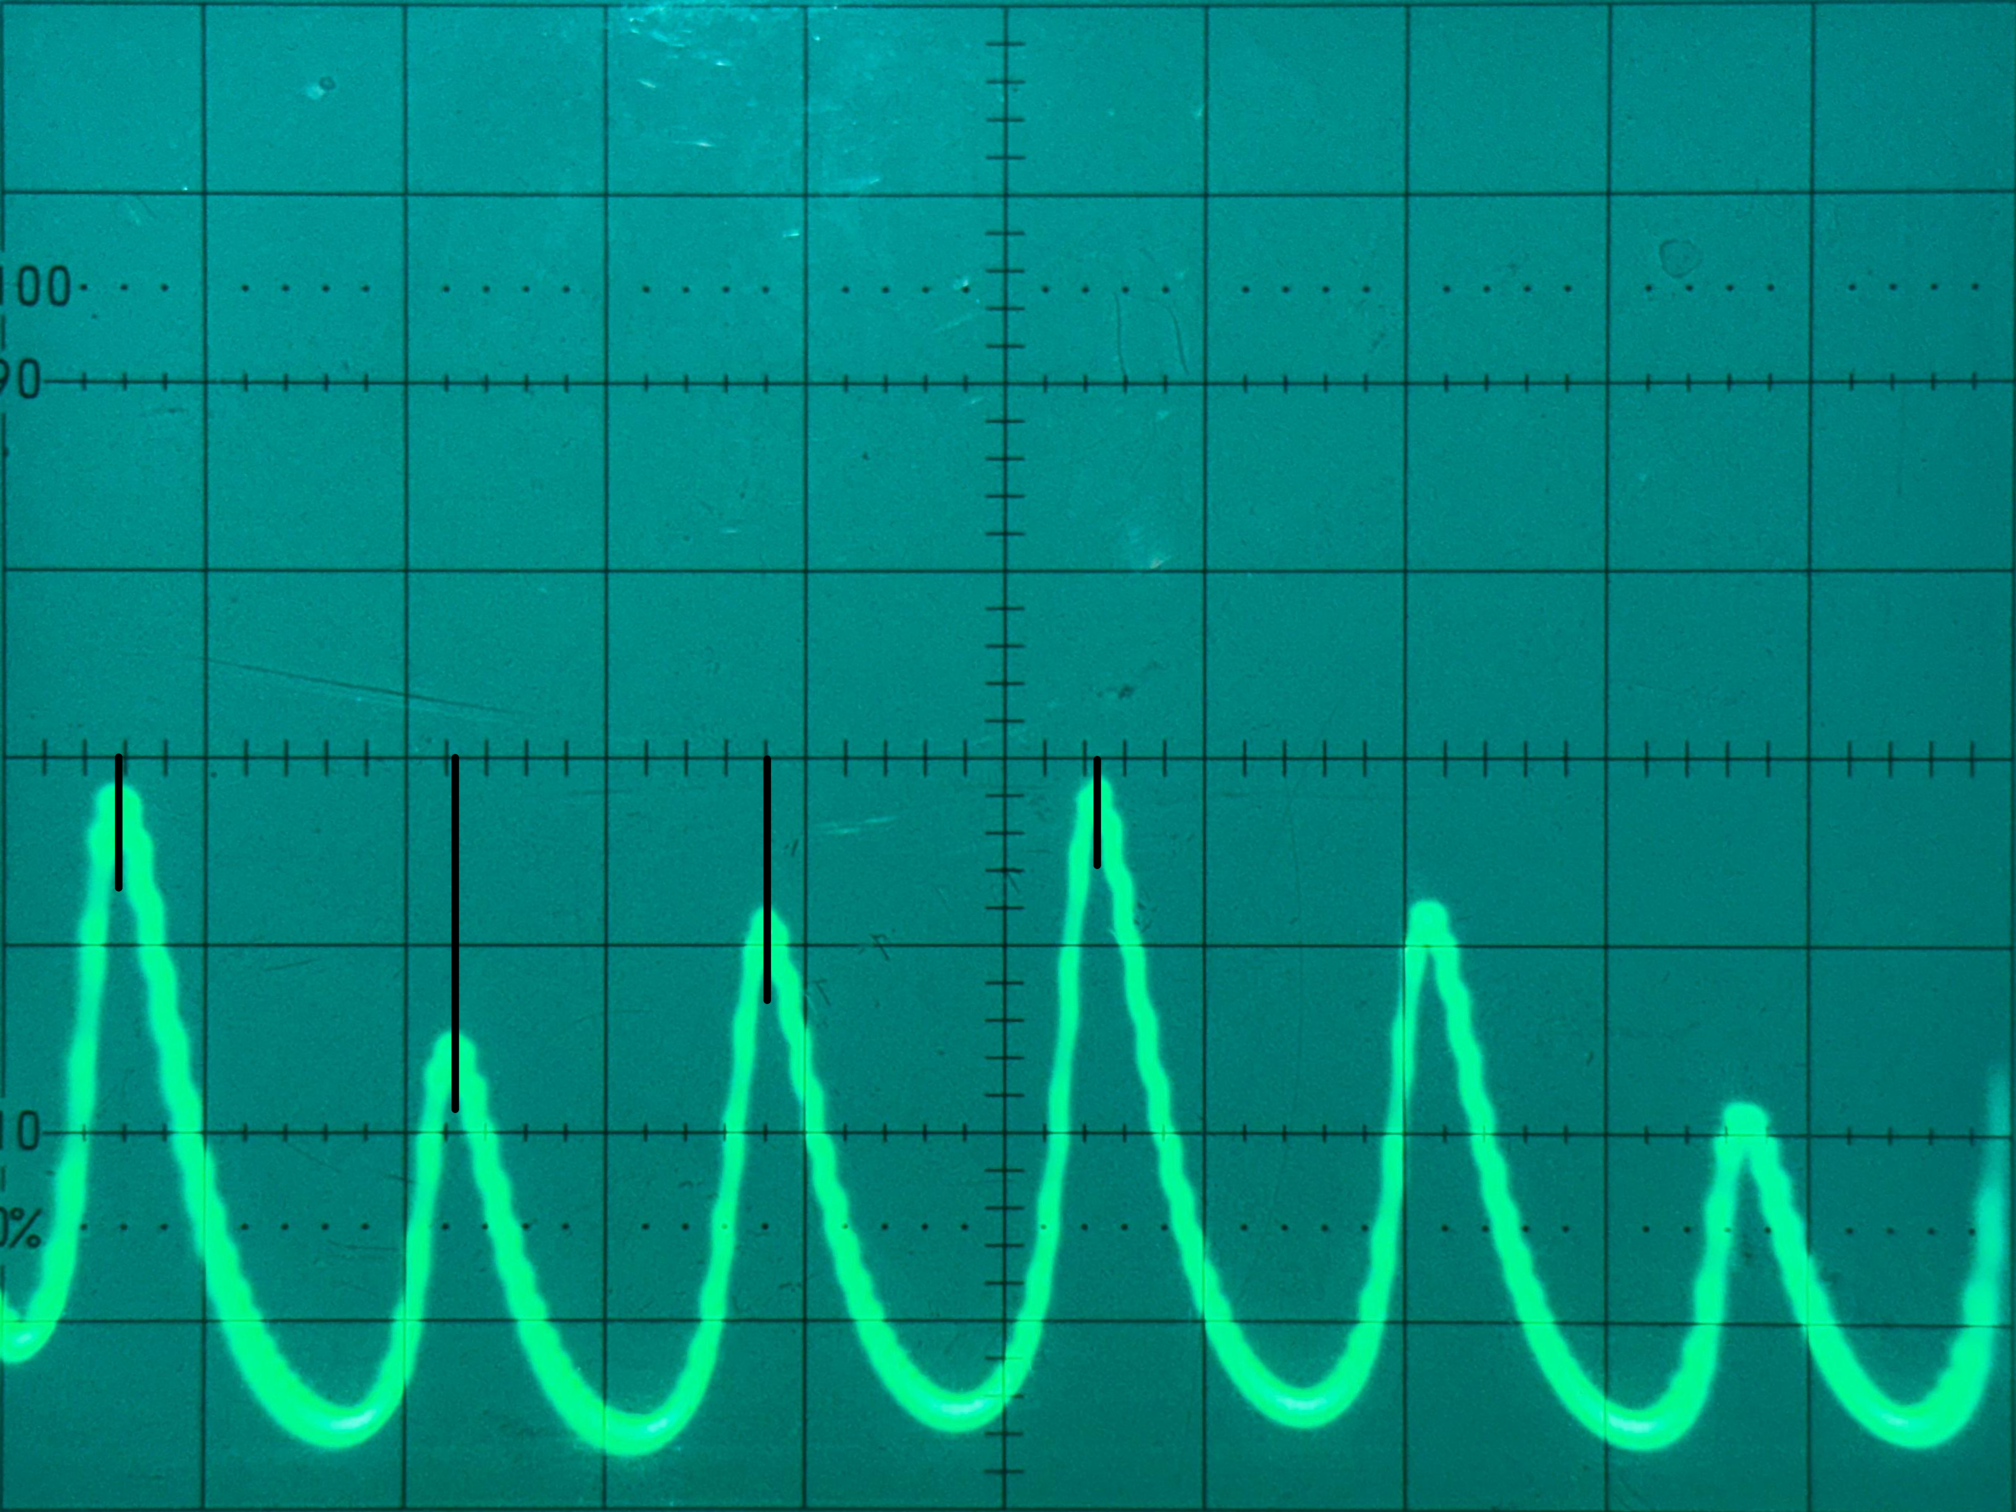
\includegraphics[width=\textwidth]{analysator-lang}
    \subcaption{mit Laserresonator der Länge L=\SI{61.5}{\cm}.}
    \label{fig:analysator-lang}
  \end{subfigure}
  \caption{
    Oszilloskop-Bilder des Spektrumanalysators. Es sind Hilfslinien zum besseren Ablesen eingezeichnet.
    Bei Betrachtung mit dem Auge sieht man jeweils eine zweite Linie,
    welche der hier erkennbaren überlagert und horizontal verschoben ist.
    Die zwei Linien entsprechen vermutlich dem Hin- und Rückweg (d.h. der Verlängerung und Verkürzung) des Piezos, die sich
    durch Hysterese-Effekte leicht voneinander unterscheiden.}
  \label{fig:analysator}
\end{figure}
Bei genügend hoher Piezo-Spannungsamplitude ist zu erwarten, dass sich die Länge des Analysators stark genug ändert,
dass er zweimal die gleiche Resonanzfrequenz hat (z.B. $\nu_{qnm}(l_1) = \nu_{qnm+1}(l_2)$).
Dadurch ergeben sich im Oszilloskop-Bild wiederholende Strukturen. Da die hier betrachteten Längenänderungen klein
gegen die Gesamtlänge $l$ des Resonators sind, stehen Änderungen der Länge und der Resonanzfrequenz näherungsweise
in einem linearen Zusammenhang zueinander. Dann entspricht der Abstand zwischen Wiederholungen im Oszillogramm $\delta x_\mr{MD}$
dem Modenabstand $MD$ und aus den Oszillogrammen lassen sich Frequenzdifferenzen $\delta\nu$ nach dem Zusammenhang
\begin{equation}
  \frac{\delta x}{\delta x_\mr{MD}} = \frac{\delta \nu}{\mr{MD}}
\end{equation}
ablesen.

Die aus den Oszillogrammen abgelesenen Linien und deren Auswertung sind in Tab. \ref{tab:analysator} gezeigt.
\begin{figure}[h]
  \centering
  \begin{subfigure}{\textwidth}
    \centering
    \begin{tabular}{rrrrrr}
\toprule
Nr. & $x/\mathrm{Skt.}$ & $\delta\nu/\mathrm{FSR}$ & $\Delta\delta\nu/\mathrm{FSR}$ & $\delta\nu$ & $\Delta\delta\nu$ \\
\midrule
1 & -9.1 & - & - & - & - \\
2 & -0.4 & 0.000 & 0.045 & - & - \\
3 & 2.0 & 0.253 & 0.0461 & 379 & 69 \\
4 & 7.4 & 0.821 & 0.0578 & 1231 & 87 \\
5 & 9.1 & 1.000 & 0.0632 & - & - \\
6 & 18.5 & - & - & - & - \\
\bottomrule
\end{tabular}

    \subcaption{
      L=\SI{48.6}{\cm}, Positionen $x$ abgelesen aus Abb. \ref{fig:analysator-kurz}.
      Es ist hier nicht direkt ersichtlich, welche Distanz dem Modenabstand entspricht.
      Da Linien 1, 2, 5 und 6 etwa gleich weit voneinander entfernt sind, wird diese Distanz mit dem Modenabstand identifiziert.
      Die Dazwischen erkennbaren Moden sind dann Linien 3 und 4.
      }
    \label{tab:analysator-kurz}
  \end{subfigure}

  \begin{subfigure}{\textwidth}
    \centering
    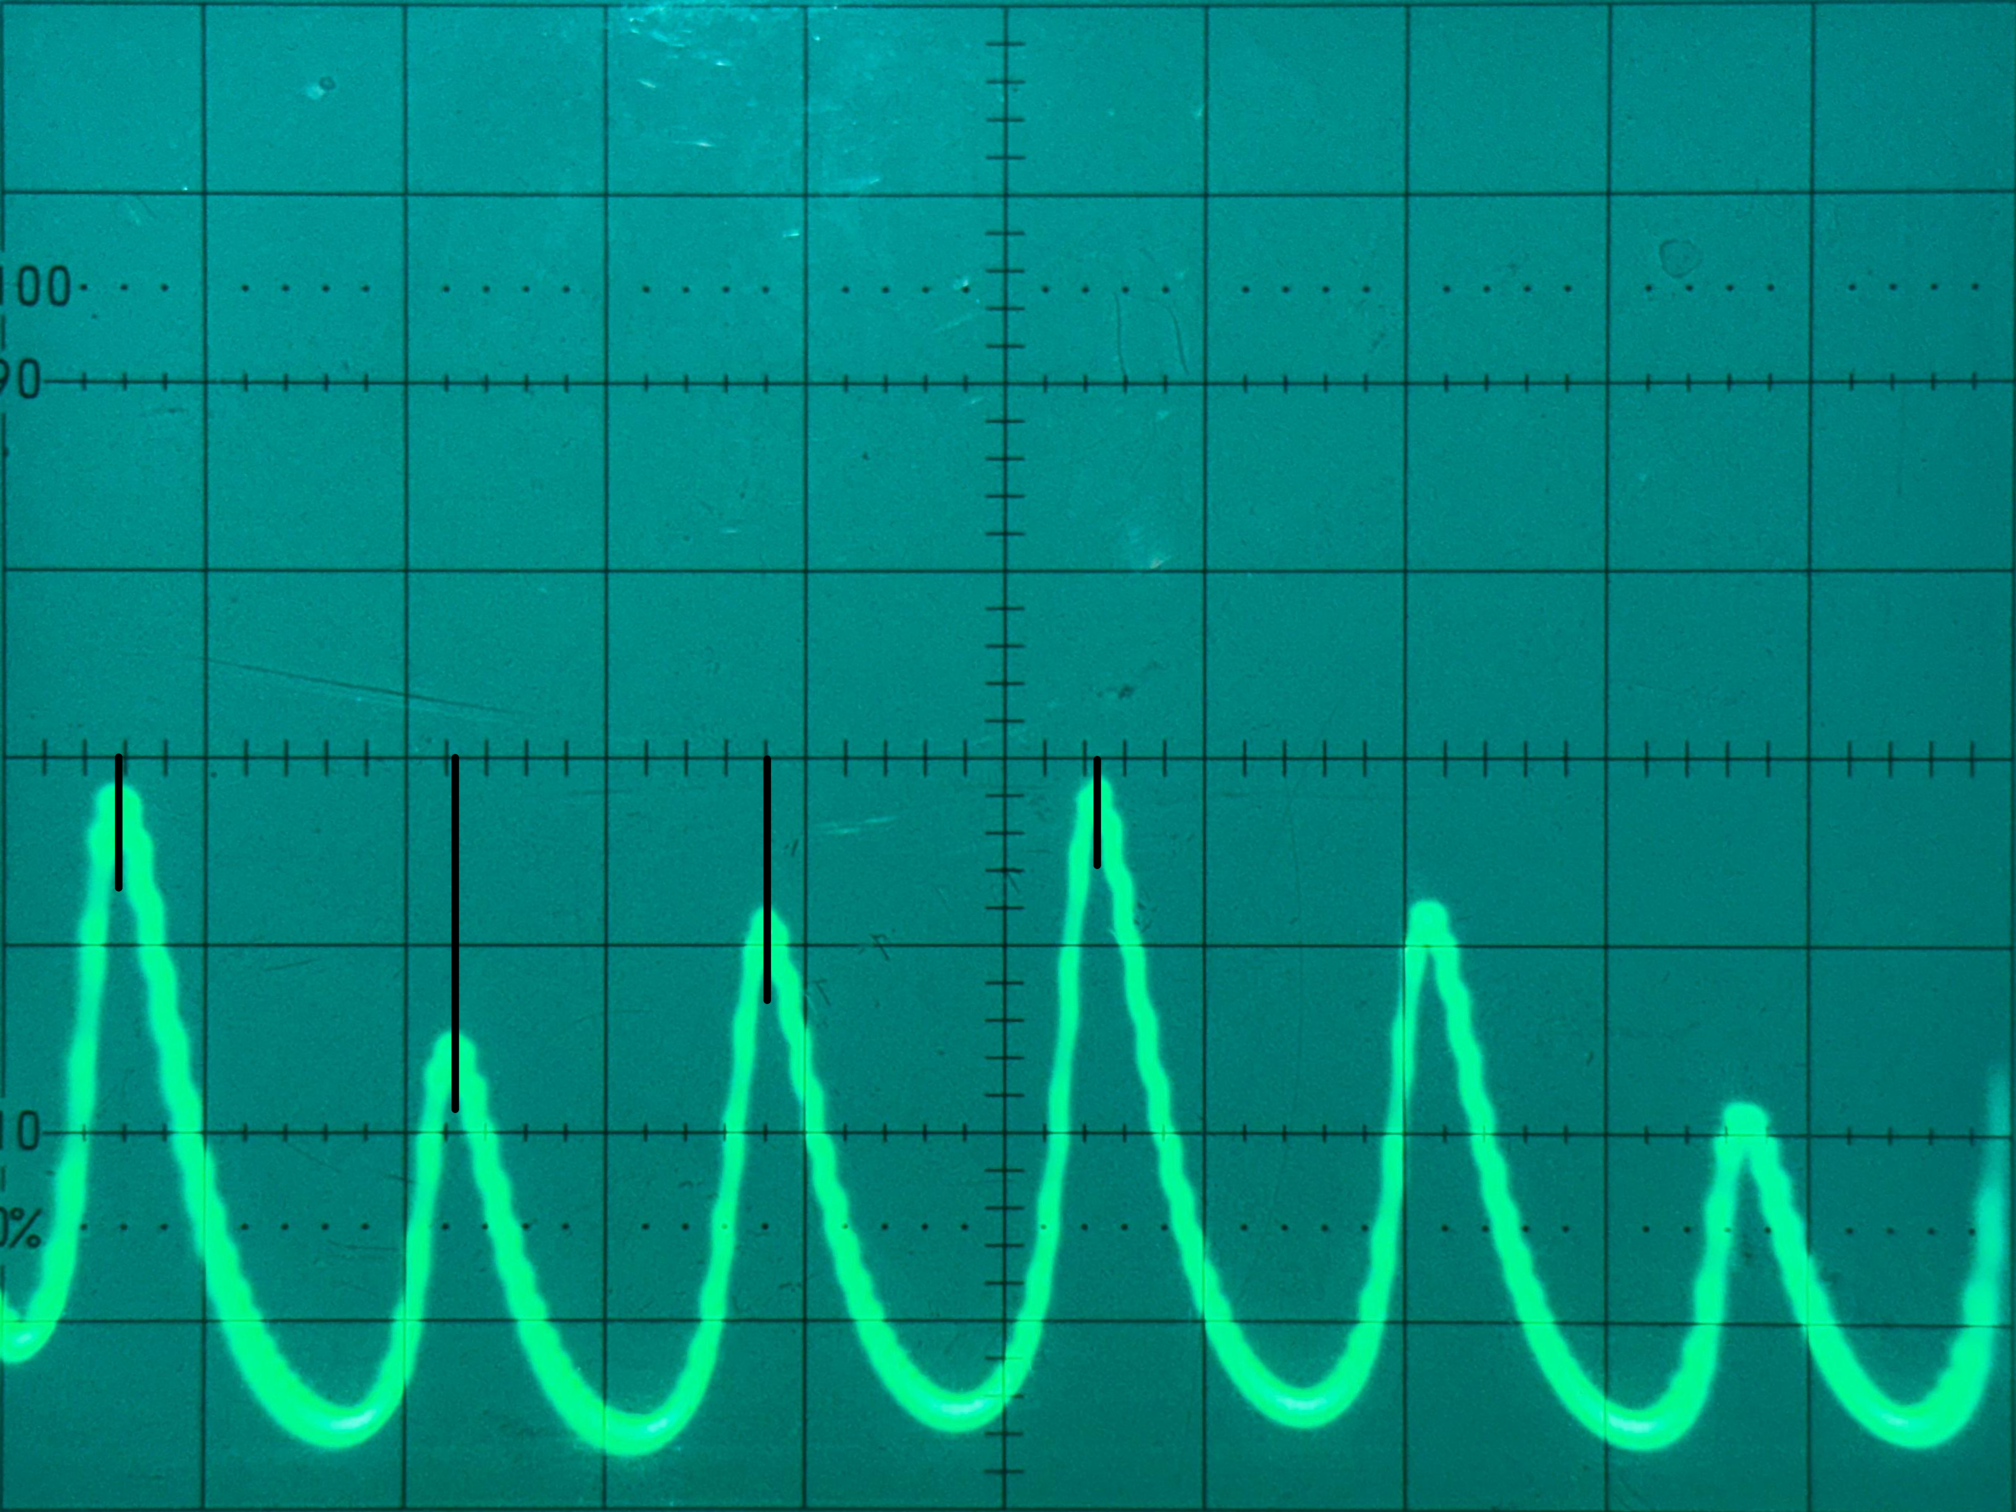
\includegraphics[width=\textwidth]{analysator-lang}
    \subcaption{L=\SI{61.5}{\cm}, Positionen $x$ abgelesen aus Abb. \ref{fig:analysator-lang}.}
    \label{tab:analysator-lang}
  \end{subfigure}
  \caption{
    Aus den Oszillogrammen des Spektrumanalysators abgelesene Linien. $\Delta x = 0.3\mr{Skt.}$ und $\delta\nu$ ist in \si\MHz angegeben.}
  \label{tab:analysator}
\end{figure}





\clearpage
\section{Fazit}



\clearpage
\section{Anhang}



\clearpage
\begin{thebibliography}{9}

\bibitem{Anleitung}
\textit{Physikalisches Praktikum Teil IV -- Versuchsbeschreibungen}, Universität Bonn, 10.10.2024



\end{thebibliography}

\end{document}

